\documentclass[11pt]{article}
\usepackage{graphicx}
\usepackage{listings}
\usepackage{courier}
\usepackage[pdfborder=0 0 0]{hyperref}
\usepackage{url}
\usepackage[cm]{fullpage}
\newcommand{\HRule}{\rule{\linewidth}{0.5mm}}
\setlength{\parindent}{0cm}
\setlength{\parskip}{0.3cm}
\begin{document}
\title{DRAMSim2}
\author{Elliott Cooper-Balis \\
			Paul Rosenfeld \\
			Bruce Jacob \\
			University of Maryland \\
			\texttt{\footnotesize dramninjas \textit{[at]} gmail \textit{[dot]} com}
}
\date{}
\maketitle
\HRule
\tableofcontents
\HRule
\lstset{basicstyle={\scriptsize\ttfamily},tabsize=2,frame=single}
\section{Why Do We Need to Simulate DRAM Systems This Accurately?}
Modern computer system performance is increasingly limited
by the performance of DRAM-based memory systems. As a result, there is great
interest in providing accurate simulations of DRAM based memory systems as part
of architectural research. Unfortunately, there is great difficulty associated
with the study of modern DRAM memory systems, arising from
the fact that DRAM-system performance depends on many
independent variables such as workload characteristics of memory access rate
and request sequence, memory-system architecture, memory-system configuration, DRAM
access protocol, and DRAM device timing parameters. As a result, system
architects and design engineers often disagree on the usefulness of a given
performance-enhancing feature, since the performance impact of that feature typically 
depends on the characteristics of specific workloads, memory-system architecture, 
memory-system configuration, DRAM access protocol and DRAM device timing parameters. 
\subsection{DRAM Scheduling Complexity is Growing}

\begin{figure}[h]
\begin{center}
\includegraphics[width=\linewidth]{docs/why1.gif}
\caption{Timing diagram showing complexity of DRAM scheduling}
\label{timingcomplex}
\end{center}
\end{figure}
Figure \ref{timingcomplex} shows the pipelined scheduling of a DDR2 SDRAM device. Despite
the fact that the simulated memory system uses a closed-page policy and 
rotates through available banks on the DRAM device, which should simplify
scheduling considerably, the scheduling of this system is actually more
complex than earlier DRAM systems: for instance, new timing parameters
such as t_{RRD} and t_{FAW} are contributing to the growing
set of timing constraints placed on each successive generation of DRAM 
devices.

\subsection{DRAM performance characteristics changes every generation}
DRAM based memory systems are impacted primarily by two attributes: 
row cycle time and device datarate. Presently, DRAM row cycle times are 
decreasing at a rate of approximately 7\% per year, and DRAM device
datarates are increasing with each new generation of DRAM devices at the rate
of 100\% every three years, 
\begin{figure}[h]
\begin{center}
\includegraphics[width=\linewidth]{docs/why2.gif}
\caption{DRAM row cycle time trends}
\label{classes}
\end{center}
\end{figure}

\begin{figure}[h]
\begin{center}
\includegraphics[width=\linewidth]{docs/why3.gif}
\caption{DRAM device data rate trends}
\label{classes}
\end{center}
\end{figure}
The difference in the scaling trends of the DRAM device means that 
fundamental DRAM device performance characteristics are changing 
every single generation, and the changing performance characteristics
cannot be accurately predicted by linear extrapolations. The result is 
that no computer architect can rest easy knowing that he or she has 
obtained X\% of performance improvement with a set of microarchitectural
techniques on the current generation memory system, because the same set 
of microarchitectural techniques may not to be as effective in a 
future memory system due to the differences in the scaling attributes 
of DRAM devices, 

\subsection{The Sales Pitch}
Our DRAM-system simulation work enables system architects not
only to explore the impact of a set of microarchitectual techniques on a 
given memory system but also to examine the effectiveness of those 
microarchitectural techniques on a future generation memory system with
future generations of DRAM devices.

\section{About DRAMSim2}
	DRAMSim2 is a cycle accurate model of a DRAM memory controller, the DRAM
	modules which comprise system storage, and the buses by which they
	communicate. 

	The overarching goal is to have a simulator that is small,
	portable, and accurate. The simulator core has a simple interface 
	which allows it to be CPU simulator agnostic and should to work with any simulator (see section \ref{library}).  This core has no external run
	time or build time dependencies and has been tested with g++ on Linux
	as well as g++ on Cygwin on Windows.  

\section{Getting DRAMSim2}

DRAMSim2 is available on \href{http://github.com/dramninjasUMD}{github}. If you have git installed you can clone our repository by typing:\\

\texttt{\$ git clone git://github.com/dramninjasUMD/DRAMSim2.git }



\section{Building DRAMSim2}
	To build an optimized standalone trace-based simulator called \texttt{DRAMSim} simply type:

	\texttt{\$ make}

	For a debug build which contains debugging symbols and verbose output, run:

	\texttt{\$ make DEBUG=1}

	To build the DRAMSim2 library, type: 

	\texttt{\$ make libdramsim.so }

\section{Running DRAMSim2}
\begin{minipage}{\textwidth}
\subsection{Trace-Based Simulation}

In standalone mode, DRAMSim2 can simulate memory system traces. While traces are not as accurate
as a real CPU model driving the memory model, they are convenient since they can be generated in a number of different
ways (instrumentation, hardware traces, CPU simulation, etc.) and reused. 

We've provided a few small sample traces in the \texttt{traces/} directory. These gzipped
traces should first be pre-processed before running through the simulator. 
To run the preprocessor (the preprocessor requires python): 
\begin{lstlisting}
cd traces/
./traceParse.py k6_aoe_02_short.trc.gz
\end{lstlisting}
	This should produce the file \texttt{traces/k6\_aoe\_02\_short.trc}. Then, go back to the DRAMSim2 directory and run the trace based simulator:

\begin{lstlisting}
cd .
./DRAMSim -t traces/k6_aoe_02_short.trc -s system.ini -d ini/DDR3_micron_64M_8B_x4_sg15.ini -c 1000
\end{lstlisting}
	This will run a 1000 cycle simulation of the \texttt{k6\_aoe\_02\_short} trace using 
	the specified DDR3 part. The -s, -d, and -t flags are required to run a simulation.

	A full list of the command line arguments can be obtained by typing:
\begin{lstlisting}
$ ./DRAMSim --help
DRAMSim2 Usage: 
DRAMSim -t tracefile -s system.ini -d ini/device.ini [-c #] [-p pwd] -q
	-t, --tracefile=FILENAME 	specify a tracefile to run  
	-s, --systemini=FILENAME 	specify an ini file that describes the memory system parameters  
	-d, --deviceini=FILENAME 	specify an ini file that describes the device-level parameters
	-c, --numcycles=# 		specify number of cycles to run the simulation for [default=30] 
	-q, --quiet 			flag to suppress simulation output (except final stats) [default=no]
	-o, --option=OPTION_A=234			overwrite any ini file option from the command line
	-p, --pwd=DIRECTORY		Set the working directory

\end{lstlisting}

	Some traces include timing information, which can be used
	by the simulator or ignored. The benefit of ignoring timing information is that requests
	will stream as fast as possible into the memory system and can serve as a good stress
	test. To toggle the use of clock cycles, please change the \texttt{useClockCycle} flag in \texttt{TraceBasedSim.cpp}.

	If you have a custom trace format you'd like to use, you can modify the \texttt{parseTraceFileLine()} function ton add
	support for your own trace formats. 

	The prefix of the filename determines which type of trace this function will use (ex: k6\_foo.trc) will use the k6 format 
	in \texttt{parseTraceFileLine()}.
\end{minipage}

\subsection{Library Interface}\label{library}
In addition to simulating memory traces, DRAMSim2 can also be built as a dynamic
shared library which is convenient for connecting it to CPU simulators or other
custom front ends.  A \texttt{MemorySystem} object encapsulates the
functionality of the memory system (i.e., the memory controller and DIMMs). The 
classes that comprise DRAMSim2 can be seen in figure \ref{classes}. A
simple example application is provided in the \texttt{example\_app/} directory.
At this time we have plans to provide code to integrate DRAMSim2 into 
\href{http://www.marss86.org/index.php/Home}{MARSSx86},
\href{http://www.cs.sandia.gov/sst/}{SST}, and (eventually)
\href{http://www.m5sim.org/}{M5}.

\begin{figure}[h]
\begin{center}
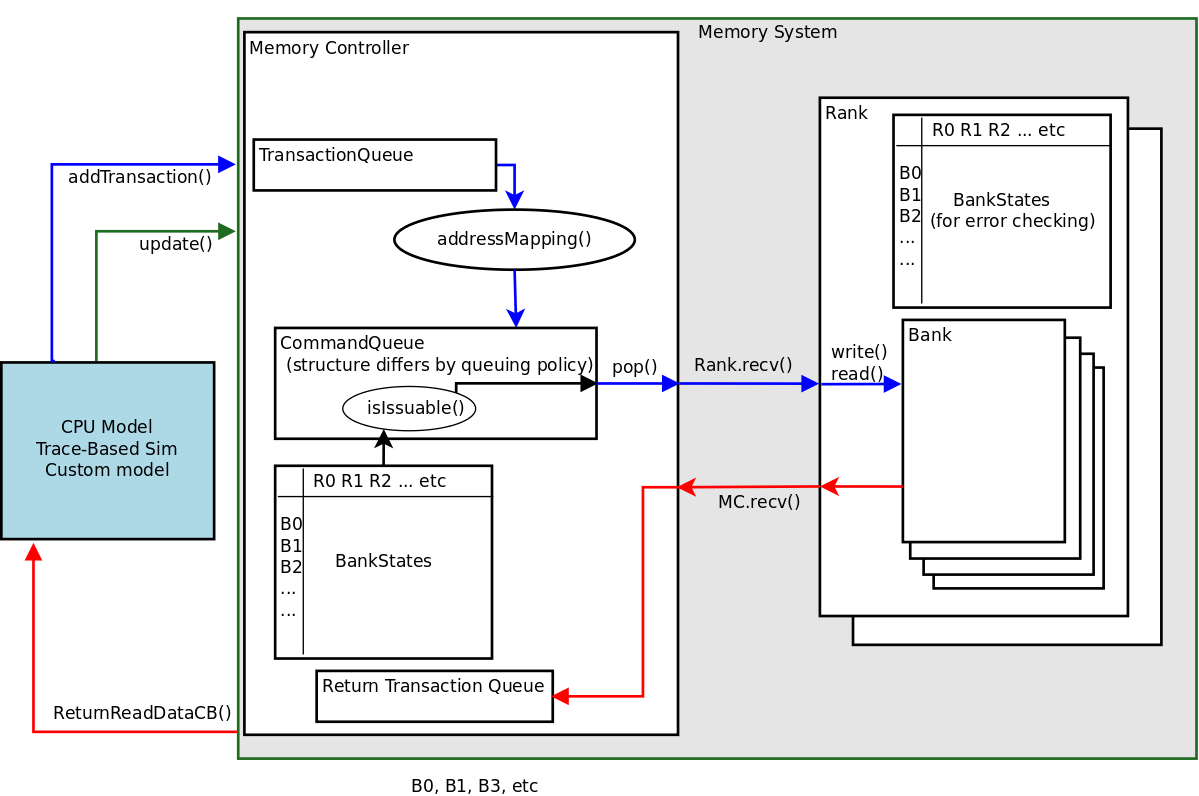
\includegraphics[width=\linewidth]{docs/classes.png}
\caption{Block diagram of DRAMSim2. The \texttt{\footnotesize recv()} functions are actually called
\texttt{\footnotesize receiveFromBus()} but were abbreviated to save sapce.}
\label{classes}
\end{center}
\end{figure}

\section{Example Output}

\noindent\begin{minipage}{\textwidth}
The verbosity of the DRAMSim2 can be customized in the system.ini file by turning the
various debug flags on or off. 

Below, we have provided a detailed explanation of the simulator output.  With
all DEBUG flags enabled, the following output is displayed for each cycle
executed.  

   \textbf{NOTE} : BP = Bus Packet, T  = Transaction \\ 
					MC = MemoryController, R\# = Rank (index \#)
  
\begin{lstlisting}
 ----------------- Memory System Update ------------------
 ---------- Memory Controller Update Starting ------------ [8]
 -- R0 Receiving On Bus    : BP [ACT] pa[0x5dec7f0] r[0] b[3] row[1502] col[799]
 -- MC Issuing On Data Bus    : BP [DATA] pa[0x7edc7e0] r[0] b[2] row[2029] col[799] data[0]=
 ++ Adding Read energy to total energy
 -- MC Issuing On Command Bus : BP [READ_P] pa[0x5dec7f8] r[1] b[3] row[1502] col[799]
== New Transaction - Mapping Address [0x5dec800] (read)
  Rank : 0
  Bank : 0
  Row  : 1502
  Col  : 800
 ++ Adding IDD3N to total energy [from rank 0]
 ++ Adding IDD3N to total energy [from rank 1]
== Printing transaction queue
  8]T [Read] [0x45bbfa4]
  9]T [Write] [0x55fbfa0] [5439E]
  10]T [Write] [0x55fbfa8] [1111]
== Printing bank states (According to MC)
[idle] [idle] [2029] [1502] 
[idle] [idle] [1502] [1502] 

== Printing Per Rank, Per Bank Queue
 = Rank 0
    Bank 0   size : 2
       0]BP [ACT] pa[0x5dec800] r[0] b[0] row[1502] col[800]
       1]BP [READ_P] pa[0x5dec800] r[0] b[0] row[1502] col[800]
    Bank 1   size : 2
       0]BP [ACT] pa[0x5dec810] r[0] b[1] row[1502] col[800]
       1]BP [READ_P] pa[0x5dec810] r[0] b[1] row[1502] col[800]
    Bank 2   size : 2
       0]BP [ACT] pa[0x5dec7e0] r[0] b[2] row[1502] col[799]
       1]BP [READ_P] pa[0x5dec7e0] r[0] b[2] row[1502] col[799]
    Bank 3   size : 1
       0]BP [READ_P] pa[0x5dec7f0] r[0] b[3] row[1502] col[799]
 = Rank 1
    Bank 0   size : 2
       0]BP [ACT] pa[0x5dec808] r[1] b[0] row[1502] col[800]
       1]BP [READ_P] pa[0x5dec808] r[1] b[0] row[1502] col[800]
    Bank 1   size : 2
       0]BP [ACT] pa[0x5dec818] r[1] b[1] row[1502] col[800]
       1]BP [READ_P] pa[0x5dec818] r[1] b[1] row[1502] col[800]
    Bank 2   size : 1
       0]BP [READ_P] pa[0x5dec7e8] r[1] b[2] row[1502] col[799]
    Bank 3   size : 0
\end{lstlisting}
\end{minipage}

\begin{minipage}{\textwidth}
Anything sent on the bus is encapsulated in an BusPacket (BP) object. When
printing, they display the following information:
\begin{lstlisting}
BP [ACT] pa[0x5dec818] r[1] b[1] row[1502] col[800]
\end{lstlisting}
The information displayed  is (in order): command type, physical address, rank
\#, bank \#, row \#, and column \#.
\end{minipage}


\begin{minipage}{\textwidth}
Lines beginning with " -- " indicate bus traffic, ie, 
\begin{lstlisting}
     -- R0 Receiving On Bus       : BP [ACT] pa[0x5dec7f0] r[0] b[3] row[1502] col[799]
     -- MC Issuing On Data Bus    : BP [DATA] pa[0x7edc7e0] r[0] b[2] row[2029] col[799] data[0]=
     -- MC Issuing On Command Bus : BP [READ_P] pa[0x5dec7f8] r[1] b[3] row[1502] col[799]
\end{lstlisting}
Sender and receiver are indicated and the packet being sent is detailed.
\end{minipage}

Lines beginning with " ++ " indicate power calculations, ie, 
\begin{lstlisting}
		 ++ Adding Read energy to total energy
 		 ++ Adding IDD3N to total energy [from rank 0]
 		 ++ Adding IDD3N to total energy [from rank 1]
\end{lstlisting}
The state of the system and the actions taken determine which current draw is used. For further detail about each current value, see Micron datasheet.  


If a pending transaction is in the transaction queue, it will be printed, as seen below:
\begin{lstlisting}
	 == Printing transaction queue		
		1]T [Read] [0x45bbfa4]
		2]T [Write] [0x55fbfa0] [5439E]
		3]T [Write] [0x55fbfa8] [1111]
\end{lstlisting}
Currently, at the start of every cycle, the head of the transaction
queue is removed, broken up into DRAM commands and placed in the
appropriate command queues.  To do this, an address mapping scheme
is applied to the transaction's physical address, the output of 
which is seen below:
\begin{lstlisting}
	== New Transaction - Mapping Address [0x5dec800] (read)
	 Rank : 0
		 Bank : 0
		 Row  : 1502
		 Col  : 800
\end{lstlisting}

If there are pending commands in the command queue, they will be
printed.  The output is dependent on the designated structure for
the command queue.  For example, per-rank/per-bank queues are 
shown below:
\begin{lstlisting}
   = Rank 1
    Bank 0   size : 2
       0]BP [ACT] pa[0x5dec808] r[1] b[0] row[1502] col[800]
       1]BP [READ_P] pa[0x5dec808] r[1] b[0] row[1502] col[800]
    Bank 1   size : 2
       0]BP [ACT] pa[0x5dec818] r[1] b[1] row[1502] col[800]
       1]BP [READ_P] pa[0x5dec818] r[1] b[1] row[1502] col[800]
    Bank 2   size : 1
       0]BP [READ_P] pa[0x5dec7e8] r[1] b[2] row[1502] col[799]
    Bank 3   size : 0
\end{lstlisting}

The state of each bank in the system is also displayed:
\begin{lstlisting}
    == Printing bank states (According to MC)
    [idle] [idle] [2029] [1502] 
    [idle] [idle] [1502] [1502] 
\end{lstlisting}
Banks can be in many states, including idle, row active (shown
with the row that is active), refreshing, or precharging.  These
states will update based on the commands being sent by the 
controller.  

\section{Results Output}

In addition to printing memory statistics and debug information to standard out, DRAMSim2 also produces
a 'vis' file in the \texttt{results/} directory. A vis file is essentially a summary of relevant statistics that is generated
per epoch (the number of cycles per epoch can be set by changing the \texttt{EPOCH\_COUNT} parameter in the \texttt{system.ini} file). 

We are currently working on DRAMVis, which is a cross-platform viewer which parses the vis file and generates graphs that can be used
to analyze and compare results.

\end{document}
